\chapter{}
\section{Energy Scale and Resolution Measurements}
\label{app:escaleandresolutiontabs}

The energy scale and resolution is measured in the 2011 dataset using $\Zee$ events as 
described in Section~\ref{sec:superclusterenergyreconstruction}. 
The additional resolution required to match the 
$\Zee$ peak in MC to that of the data (Table~\ref{tab:eres2011}) is used to correct the 
Higgs MC for modelling the signal in the $\Hgg$ analysis.
The scale measurements (Tables~\ref{tab:escale2011eb} and~\ref{tab:escale2011ee} ) are used to correct the energy of the
photons in data. 
\begin{table}[hbt]
\centering
  \begin{tabular}{|c|c|}
    \hline
    Category    			& 	$\sigma_E/E$ (\%)     	  \\
    \hline				  			      
    EB, $\abs{\eta} < 1$, $R9 > 0.94$, NOT GAP  & 	$0.67^{+0.10}_{-0.33} \pm 0.22$ \\
    EB, $\abs{\eta} < 1$, $R9 > 0.94$, GAP  	& 	$0.77^{+0.06}_{-0.12} \pm 0.22$ \\
    EB, $\abs{\eta} < 1$, $R9 < 0.94$  	& 	$0.96^{+0.05}_{-0.05} \pm 0.24$ \\
    EB, $\abs{\eta} > 1$, $R9 > 0.94$ 	& 	$1.41^{+0.15}_{-0.33} \pm 0.60$ \\
    EB, $\abs{\eta} > 1$, $R9 < 0.94$ 	&  	$1.96^{+0.06}_{-0.07} \pm 0.59$ \\
    \hline				  			      			     		     
    EE, $\abs{\eta} < 2$, $R9 > 0.94$  	& 	$2.68^{+0.15}_{-0.20} \pm 0.90$\\
    EE, $\abs{\eta} < 2$, $R9 < 0.94$  	& 	$2.79^{+0.09}_{-0.10} \pm 0.30$\\
    EE, $\abs{\eta} > 2$, $R9 > 0.94$ 	& 	$2.93^{+0.08}_{-0.08} \pm 0.34$\\
    EE, $\abs{\eta} > 2$, $R9 < 0.94$ 	& 	$3.01^{+0.11}_{-0.12} \pm 0.52$\\
    
    \hline
  \end{tabular}
\caption{Additional energy resolution  included in the $\Hgg$ signal model measured
from comparison of $\Zee$ data and MC. 
The label ``NOT GAP'' indicates 
superclusters whose seed crystal is located more 
than 5 crystals away from an ECAL module
boundary whereas the label ``GAP'' indicates superclusters whose seed crystal is within 5 crystals of an ECAL module boundary~\citep{AN-12-160}.}
\label{tab:eres2011}
\end{table} 

\begin{table}[hbt]
\centering
\begin{tabular}{|c|c|c|}
\hline
Category & Run Range & $\Delta P$ \\
\hline
EB, $ \abs{\eta} < 1 $, $\rnine < 0.94$ & 160431 - 167913 & $ -0.0004 \pm 0.0002 \pm 0.0019$ \\
EB, $ \abs{\eta} < 1 $, $\rnine < 0.94$ & 170000 - 172619 & $ -0.0016 \pm 0.0002 \pm 0.0019$ \\
EB, $ \abs{\eta} < 1 $, $\rnine < 0.94$ & 172620 - 173692 & $ -0.0017 \pm 0.0002 \pm 0.0019$ \\
EB, $ \abs{\eta} < 1 $, $\rnine < 0.94$ & 175830 - 177139 & $ -0.0021 \pm 0.0002 \pm 0.0019$ \\
EB, $ \abs{\eta} < 1 $, $\rnine < 0.94$ & 177140 - 178421 & $ -0.0025 \pm 0.0002 \pm 0.0019$ \\
EB, $ \abs{\eta} < 1 $, $\rnine < 0.94$ & 178424 - 180252 & $ -0.0024 \pm 0.0002 \pm 0.0019$ \\
\hline							  		  
EB, $ \abs{\eta} < 1 $, $\rnine > 0.94$ & 160431 - 167913 & $ 0.0059 \pm 0.0002 \pm 0.0013$ \\
EB, $ \abs{\eta} < 1 $, $\rnine > 0.94$ & 170000 - 172619 & $ 0.0046 \pm 0.0002 \pm 0.0013$ \\
EB, $ \abs{\eta} < 1 $, $\rnine > 0.94$ & 172620 - 173692 & $ 0.0045 \pm 0.0002 \pm 0.0013$ \\
EB, $ \abs{\eta} < 1 $, $\rnine > 0.94$ & 175830 - 177139 & $ 0.0042 \pm 0.0002 \pm 0.0013$ \\
EB, $ \abs{\eta} < 1 $, $\rnine > 0.94$ & 177140 - 178421 & $ 0.0038 \pm 0.0002 \pm 0.0013$ \\
EB, $ \abs{\eta} < 1 $, $\rnine > 0.94$ & 178424 - 180252 & $ 0.0039 \pm 0.0002 \pm 0.0013$ \\
\hline							  		  
EB, $ \abs{\eta} > 1 $, $\rnine < 0.94$ & 160431 - 167913 & $ -0.0045 \pm 0.0006 \pm 0.0071$ \\
EB, $ \abs{\eta} > 1 $, $\rnine < 0.94$ & 170000 - 172619 & $ -0.0066 \pm 0.0008 \pm 0.0071$ \\
EB, $ \abs{\eta} > 1 $, $\rnine < 0.94$ & 172620 - 173692 & $ -0.0058 \pm 0.0007 \pm 0.0071$ \\
EB, $ \abs{\eta} > 1 $, $\rnine < 0.94$ & 175830 - 177139 & $ -0.0073 \pm 0.0006 \pm 0.0071$ \\
EB, $ \abs{\eta} > 1 $, $\rnine < 0.94$ & 177140 - 178421 & $ -0.0075 \pm 0.0006 \pm 0.0071$ \\
EB, $ \abs{\eta} > 1 $, $\rnine < 0.94$ & 178424 - 180252 & $ -0.0071 \pm 0.0007 \pm 0.0071$ \\
\hline				    			  		  
EB, $ \abs{\eta} > 1 $, $\rnine > 0.94$ & 160431 - 167913 & $ 0.0084 \pm 0.0013 \pm 0.0051$ \\
EB, $ \abs{\eta} > 1 $, $\rnine > 0.94$ & 170000 - 172619 & $ 0.0063 \pm 0.0014 \pm 0.0051$ \\
EB, $ \abs{\eta} > 1 $, $\rnine > 0.94$ & 172620 - 173692 & $ 0.0071 \pm 0.0013 \pm 0.0051$ \\
EB, $ \abs{\eta} > 1 $, $\rnine > 0.94$ & 175830 - 177139 & $ 0.0056 \pm 0.0013 \pm 0.0051$ \\
EB, $ \abs{\eta} > 1 $, $\rnine > 0.94$ & 177140 - 178421 & $ 0.0054 \pm 0.0013 \pm 0.0051$ \\
EB, $ \abs{\eta} > 1 $, $\rnine > 0.94$ & 178424 - 180252 & $ 0.0058 \pm 0.0013 \pm 0.0051$ \\
\hline
\hline
\end{tabular}
\caption{Relative energy scale difference in data and MC ($\Delta P$) in the ECAL barrel,
measured in $\Zee$ data. 
The first uncertainty given is statistical while the second is the systematic
assigned to cover the difference in the  $\rnine$ distributions between electrons
and photons~\citep{AN-12-160}.}
\label{tab:escale2011eb}
\end{table}

\begin{table}[hbt]
\centering
\begin{tabular}{|c|c|c|}
\hline
Category & Run Range & $\Delta P$ \\
\hline
EE, $ \abs{\eta} < 2 $, $\rnine < 0.94$ & 160431 - 167913 & $ -0.0082 \pm 0.0008 \pm 0.0088 $\\
EE, $ \abs{\eta} < 2 $, $\rnine < 0.94$ & 170000 - 172619 & $ -0.0025 \pm 0.0011 \pm 0.0088 $\\
EE, $ \abs{\eta} < 2 $, $\rnine < 0.94$ & 172620 - 173692 & $ -0.0035 \pm 0.0010 \pm 0.0088 $\\
EE, $ \abs{\eta} < 2 $, $\rnine < 0.94$ & 175830 - 177139 & $ -0.0017 \pm 0.0009 \pm 0.0088 $\\
EE, $ \abs{\eta} < 2 $, $\rnine < 0.94$ & 177140 - 178421 & $ -0.0010 \pm 0.0009 \pm 0.0088 $\\
EE, $ \abs{\eta} < 2 $, $\rnine < 0.94$ & 178424 - 180252 & $ 0.0030 \pm 0.0009 \pm 0.0088 $\\
\hline
EE, $ \abs{\eta} < 2 $, $\rnine > 0.94$ & 160431 - 167913 & $ -0.0033 \pm 0.0010 \pm 0.0018 $\\
EE, $ \abs{\eta} < 2 $, $\rnine > 0.94$ & 170000 - 172619 & $ 0.0024 \pm 0.0012 \pm 0.0018 $\\
EE, $ \abs{\eta} < 2 $, $\rnine > 0.94$ & 172620 - 173692 & $ 0.0014 \pm 0.0011 \pm 0.0018 $\\
EE, $ \abs{\eta} < 2 $, $\rnine > 0.94$ & 175830 - 177139 & $ 0.0032 \pm 0.0010 \pm 0.0018 $\\
EE, $ \abs{\eta} < 2 $, $\rnine > 0.94$ & 177140 - 178421 & $ 0.0040 \pm 0.0010 \pm 0.0018 $\\
EE, $ \abs{\eta} < 2 $, $\rnine > 0.94$ & 178424 - 180252 & $ 0.0079 \pm 0.0010 \pm 0.0018 $\\
\hline
EE, $ \abs{\eta} > 2 $, $\rnine < 0.94$ & 160431 - 167913 & $ -0.0064 \pm 0.0008 \pm 0.0019 $\\
EE, $ \abs{\eta} > 2 $, $\rnine < 0.94$ & 170000 - 172619 & $ -0.0046 \pm 0.0009 \pm 0.0019 $\\
EE, $ \abs{\eta} > 2 $, $\rnine < 0.94$ & 172620 - 173692 & $ -0.0029 \pm 0.0009 \pm 0.0019 $\\
EE, $ \abs{\eta} > 2 $, $\rnine < 0.94$ & 175830 - 177139 & $ -0.0040 \pm 0.0009 \pm 0.0019 $\\
EE, $ \abs{\eta} > 2 $, $\rnine < 0.94$ & 177140 - 178421 & $ -0.0050 \pm 0.0008 \pm 0.0019 $\\
EE, $ \abs{\eta} > 2 $, $\rnine < 0.94$ & 178424 - 180252 & $ -0.0059 \pm 0.0009 \pm 0.0019 $\\
\hline
EE, $ \abs{\eta} > 2 $, $\rnine > 0.94$ & 160431 - 167913 & $ 0.0042 \pm 0.0006 \pm 0.0028 $\\
EE, $ \abs{\eta} > 2 $, $\rnine > 0.94$ & 170000 - 172619 & $ 0.0060 \pm 0.0008 \pm 0.0028 $\\
EE, $ \abs{\eta} > 2 $, $\rnine > 0.94$ & 172620 - 173692 & $ 0.0077 \pm 0.0007 \pm 0.0028 $\\
EE, $ \abs{\eta} > 2 $, $\rnine > 0.94$ & 175830 - 177139 & $ 0.0067 \pm 0.0007 \pm 0.0028 $\\
EE, $ \abs{\eta} > 2 $, $\rnine > 0.94$ & 177140 - 178421 & $ 0.0056 \pm 0.0007 \pm 0.0028 $\\
EE, $ \abs{\eta} > 2 $, $\rnine > 0.94$ & 178424 - 180252 & $ 0.0047 \pm 0.0007 \pm 0.0028 $\\
\hline
\hline
\end{tabular}
\caption{Relative energy scale difference in data and MC ($\Delta P$) in the ECAL endcaps,
measured in $\Zee$ data. 
The first uncertainty given is statistical while the second is the systematic
assigned to cover the difference in the  $\rnine$ distributions between electrons
and photons~\citep{AN-12-160}.}
\label{tab:escale2011ee}
\end{table}


\clearpage
\section{Binning Algorithm Optimisation}
\label{app:binningalgooptimisation}

The optimisation procedure used to select the bin boundaries of the $\Hgg$ categorisation BDT 
involves a full scan over all combinations of bin boundaries. As this scan can be
very slow, the procedure is separated into two parts, first a broad scan in large steps 
to find the region containing the optimum point then using small steps to refine the scan.
The first step in the binning procedure is designed to ensure that at least 20 background 
events are expected in every bin. This gives a total of $B$ bins at a given luminosity.
To maintain this feature, only boundaries which match any of the $B-1$ bin edges (remembering
-1 and 1 are fixed boundaries) are scanned. The step size of the scan is therefore expressed
as a step in number of bins so that for a given BDT output range, $(b_{i},b_{j})$ includes
an integer number of the $B$ bins. The fine scan is defined to have a step size of 1,
being the minimum step size defined this way. The step size for the broad scan, $P$,
can be chosen to reduce the total time taken for the scan.
For $N$ BDT boundaries, the scan is $N$-dimensional and the total number of points to scan 
(combinations of bin boundary values) assuming the two step procedure is given by,
\begin{equation}
	\frac{\displaystyle 1}{\displaystyle 2^{N-1}} \left[ \left(\frac{\displaystyle B}{\displaystyle P}\right)^{N}
	+ (2P)^{N}\right]
\end{equation}
imposing the condition $b_{1}<b_{2}<\cdots<b_{N}$.
Figure~\ref{fig:pmin} shows the total number of iterations required to perform 
the full scan for different numbers of boundaries as a function of the broad step size
$P$. The value, $P_{min}$, which minimises the total number of iterations
is the same for any value of $N$ and is given by,
\begin{equation}
	P_{min} = e^{\frac{1}{2}\ln(B/2)}
\end{equation}
\begin{figure}
\begin{center}
  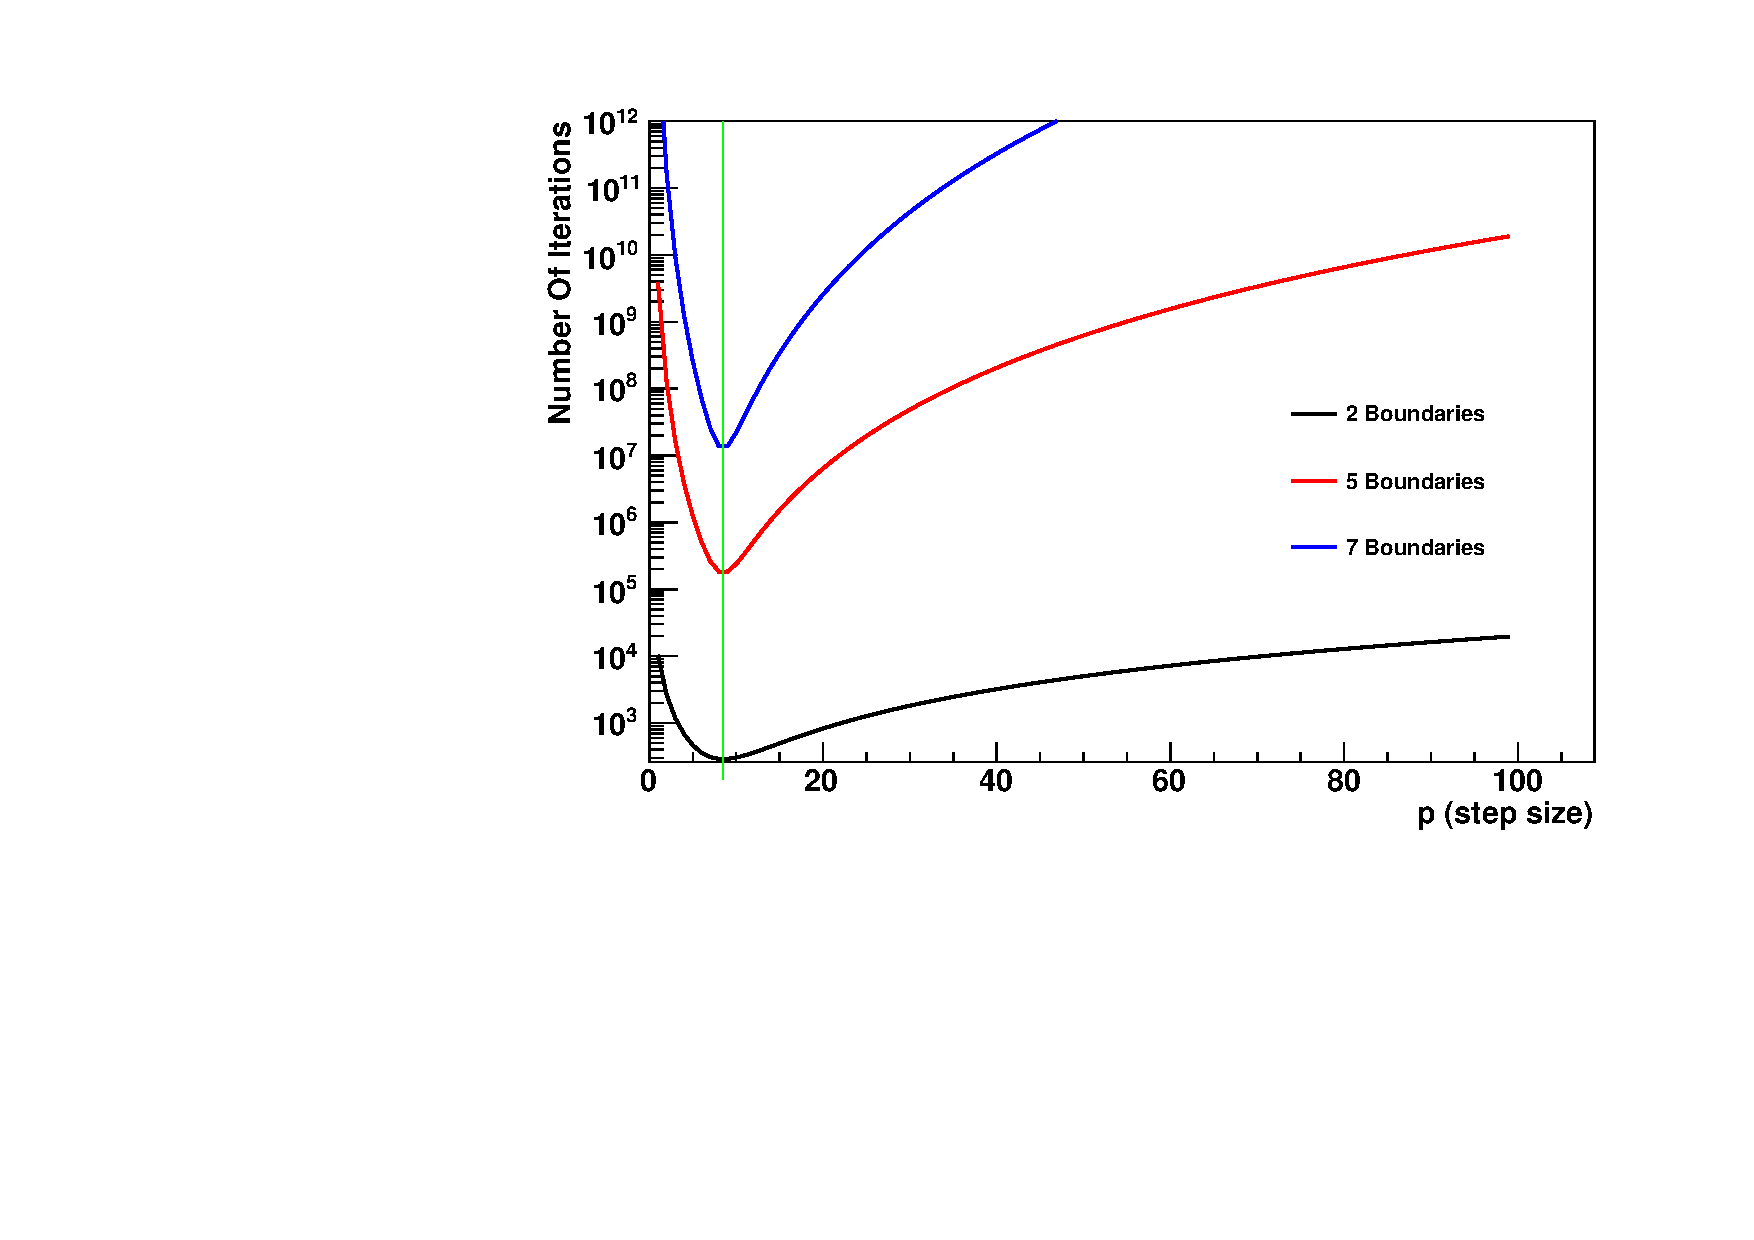
\includegraphics[width=.8\textwidth]{hgg7TeV/appendix/minimumtime.pdf}
\end{center}
 \caption{Total number of iterations in the binning optimization scan as a function of the broad step size $P$.
 The curve is shown for different numbers of final BDT boundaries. The minimum always occurs at the same 
 value of $P$ as indicated by the green vertical line.}
 \label{fig:pmin}
\end{figure}
The scan is repeated, increasing the number of boundaries until the improvement in terms of the 
maximum expected significance in the presence of a SM Higgs boson is less than 0.1\%.
Figure~\ref{fig:binningopt} shows the additional sensitivity gained as the number of final BDT output bins 
is increased for different starting values of $B$. The red curve is representative of the actual scan performed
for the 2011 analysis.

\begin{figure}
\begin{center}
  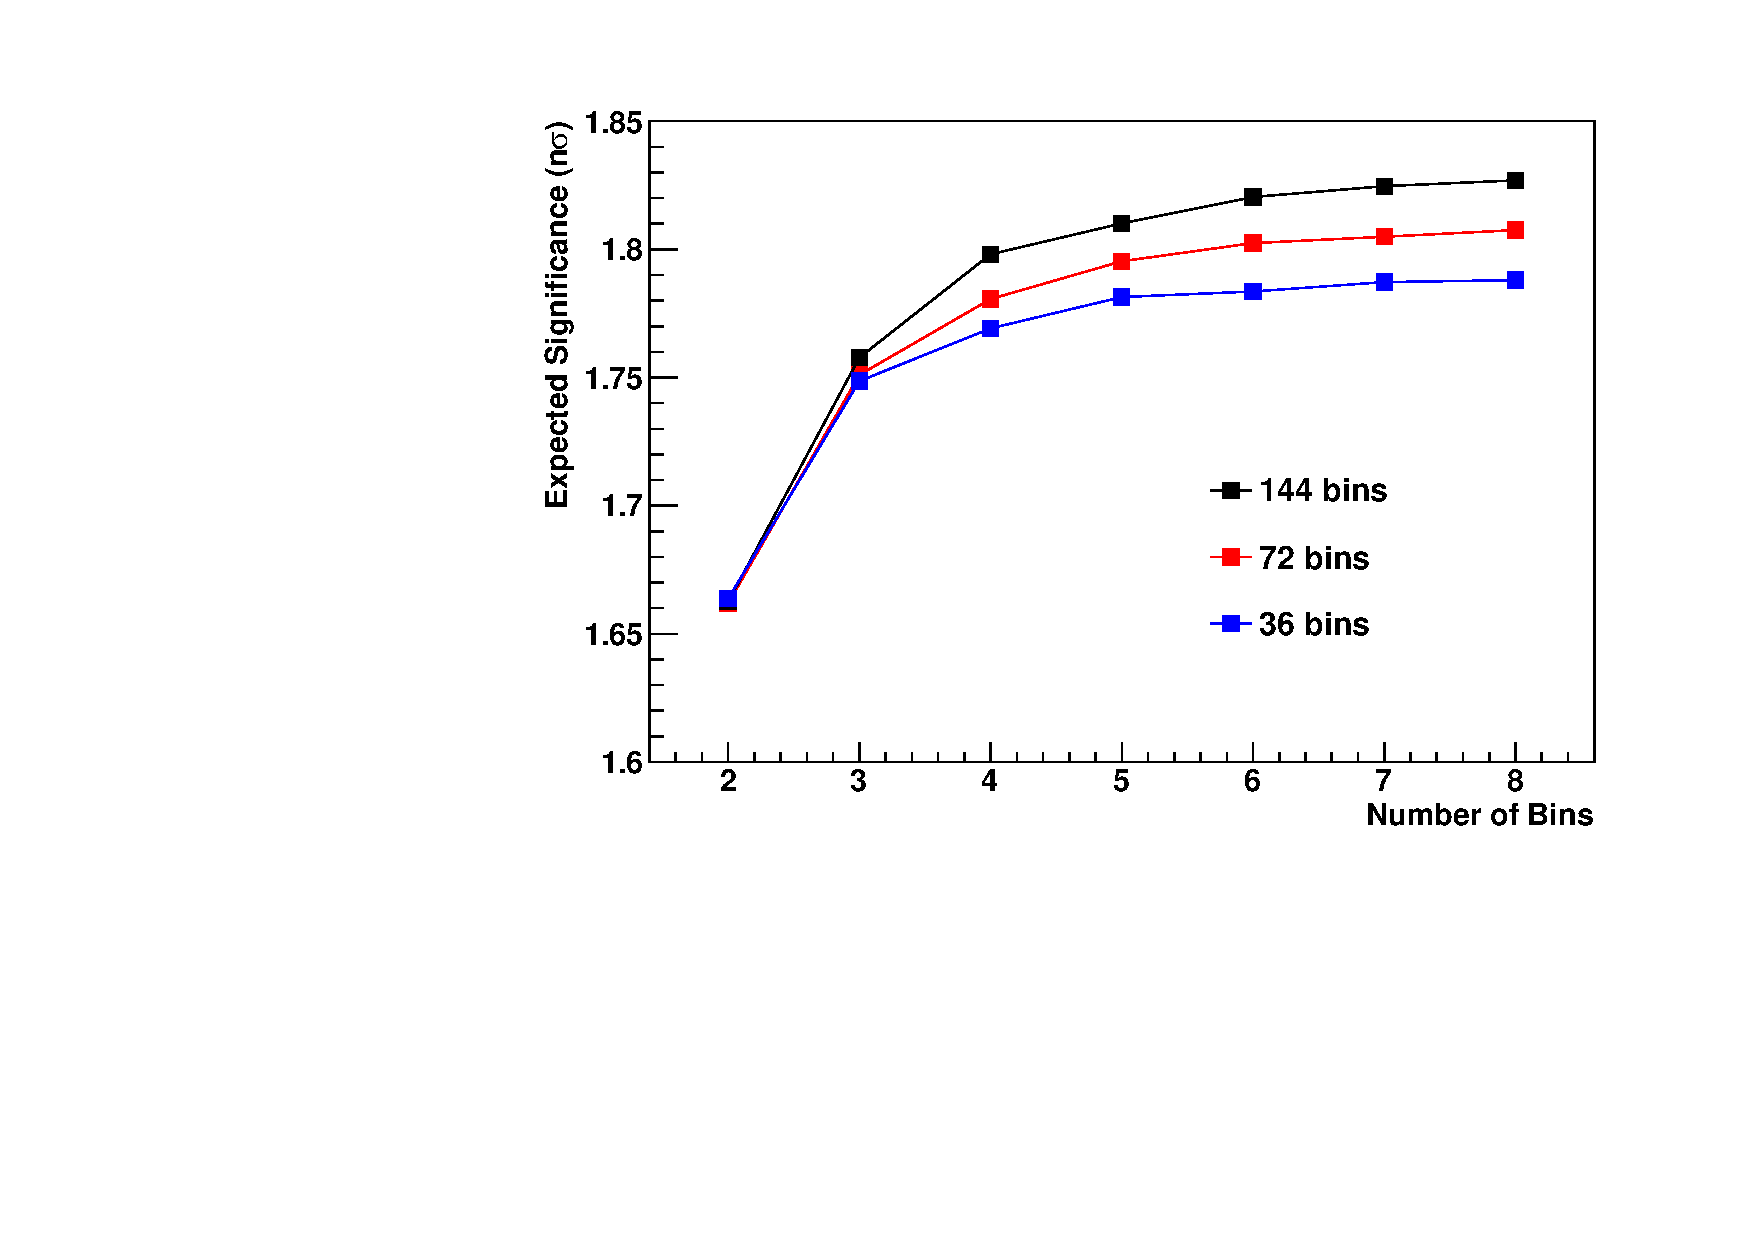
\includegraphics[width=.8\textwidth]{hgg7TeV/appendix/newbinAlgo.pdf}
\end{center}
 \caption{Increase in expected significance in the presence of a SM Higgs boson as the number of final BDT output bins
 is increased. The three curves show the improvement for different numbers of initial bins, $B$. 
 The red curve is representative of the result obtained from performing the optimization procedure in
 the 2011 analysis.}
 \label{fig:binningopt}
\end{figure}

\section{Signal Systematics}
\label{app:sigsys}

The treatment of systematic variations in the signal modelling for the $\Hgg$ analysis described in 
Chapter~\ref{chap:hgg} is the same for all uncertainties except those due to the 
theoretical uncertainty on the Higgs boson production cross-sections and the integrated luminosity measurement.
For each uncertainty, the relevant quantity in the MC is varied by 3$\sigma$ and the 
resulting BDT distributions are compared to the nominal one. The three ``templates'' (corresponding to
nominal and $\pm3\sigma$ variations) are used to determine the $1\sigma$ variations of the $j$-th BDT bin 
of the signal model due to the $k$-th signal systematic ($\sigma_{k}^{s,p}$ used in Equation~\ref{eqn:slh}).
The procedure is performed for each signal process, $p$, separately.
The value for the $1\sigma$ variation in each bin is given by,
\begin{equation}
  \sigma^{\pm} = a \pm b + c,
\end{equation}
where $\sigma^{+}$ is the value of $\sigma_{k}^{s,p}$ used for positive values of the 
associated nuisance parameter and $\sigma^{-}$ is for negative values.
The parameters $a$ and $b$ are determined for a particular bin by solving the set of simultaneous equations;
\begin{equation}
\everymath{\displaystyle}\begin{pmatrix} 
s^{-3\sigma} \\ s^{mc}  \\ s^{3\sigma}
\end{pmatrix}
=
\begin{bmatrix}
9 & -3 & 1 \\
0 & 0  & 1 \\
9 & 3  & 1
\end{bmatrix}
\begin{pmatrix} a \\ b \\ c 
\end{pmatrix},
\end{equation}
where $s^{mc}$ is the nominal value for the signal in that bin and $s^{\pm 3\sigma}$ are the values
determined from the  $\pm 3\sigma$ templates.

Figure~\ref{fig:additionalsignalsys} shows the $\pm3\sigma$ and $1\sigma$ variations
of the BDT distribution expected from the $ggH$ production process calculated from
MC and using the interpolation procedure respectively. The distributions are normalised to the expectation
in \clumi. The energy scale and resolution uncertainties can be found in Section~\ref{sec:signalmodel}
(Figure~\ref{fig:signalmodel_escaleres}).

\begin{figure}
\begin{center}
  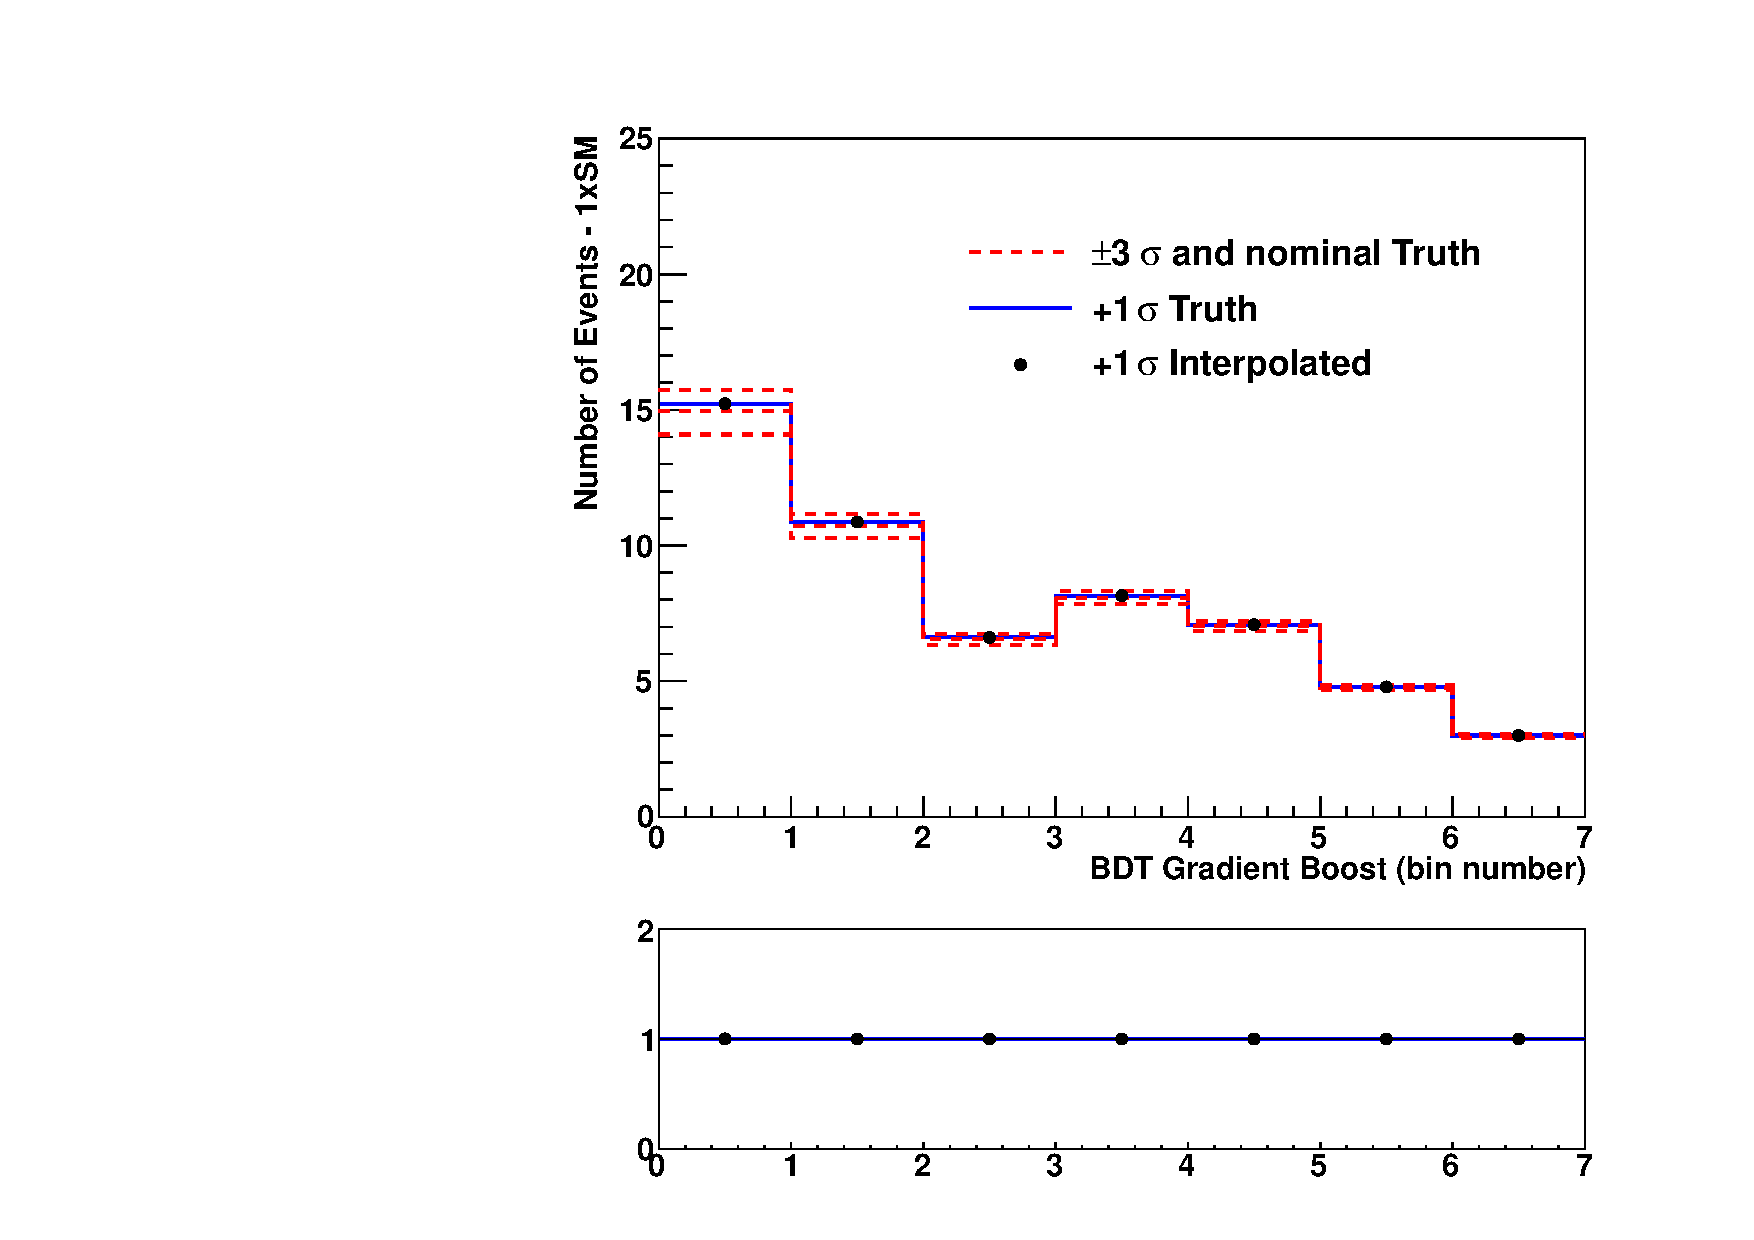
\includegraphics[width=0.45\textwidth]{hgg7TeV/sidebandMvaPlots/signalModel/systematic_interpolation_test_idEff.pdf}
  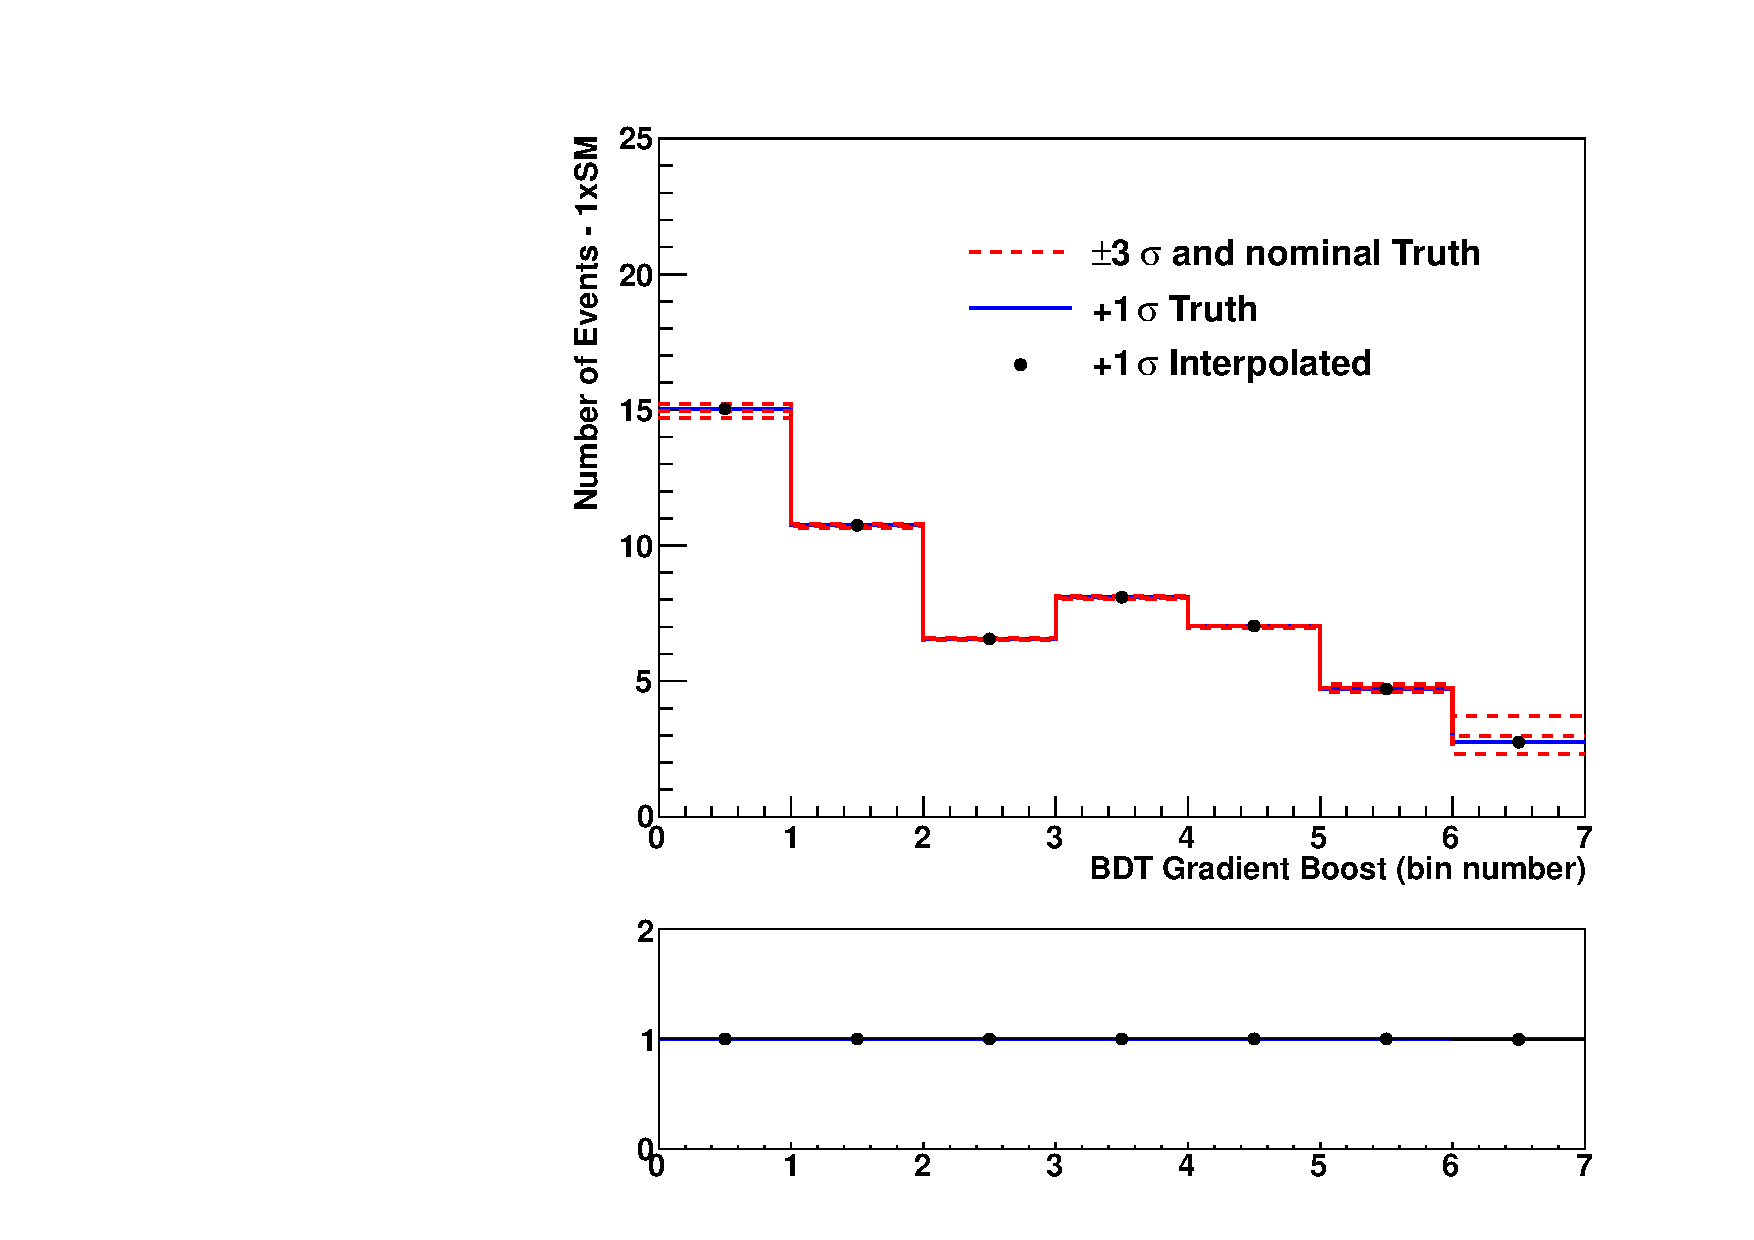
\includegraphics[width=0.45\textwidth]{hgg7TeV/sidebandMvaPlots/signalModel/systematic_interpolation_test_kFactor}\\
  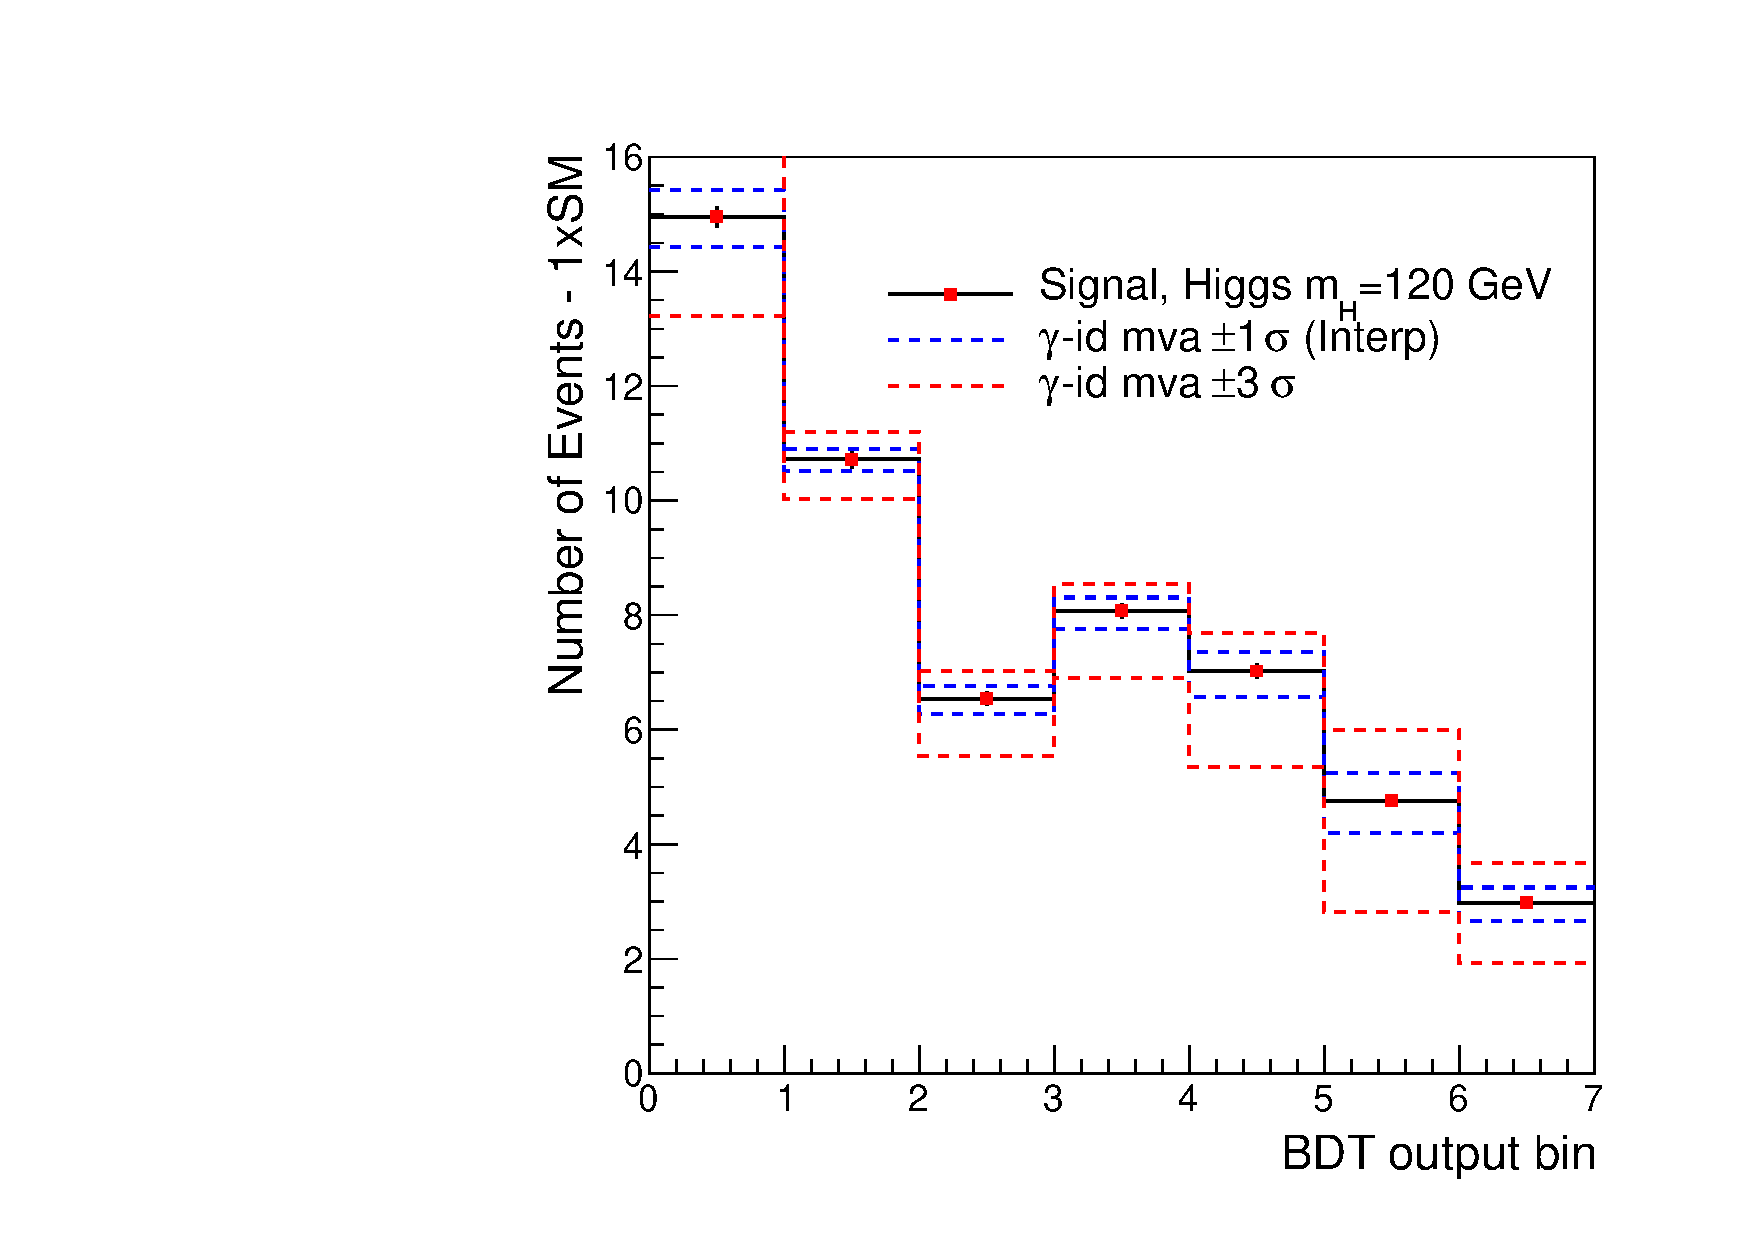
\includegraphics[width=0.45\textwidth]{hgg7TeV/sidebandMvaPlots/signalModel/systematic_interpolation_test_phoIdMva}
  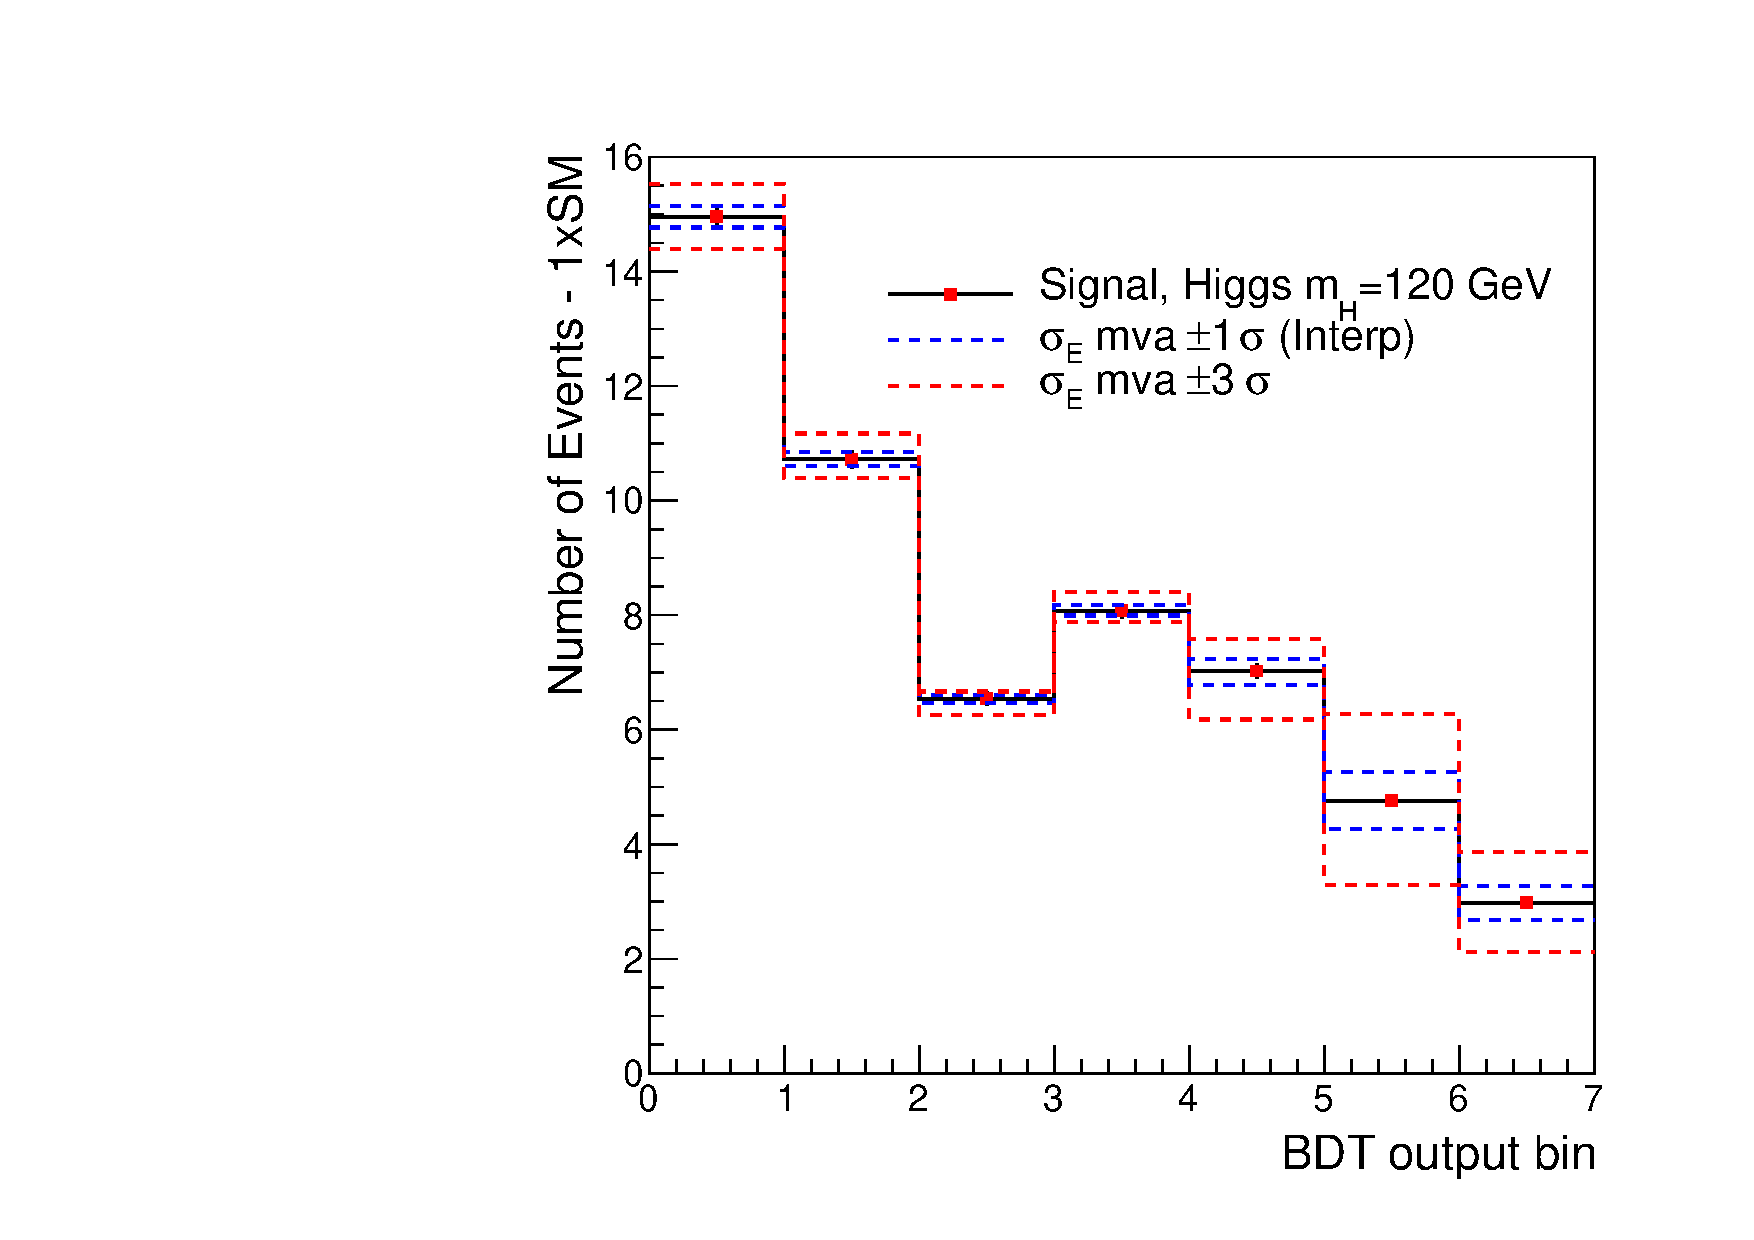
\includegraphics[width=0.45\textwidth]{hgg7TeV/sidebandMvaPlots/signalModel/systematic_interpolation_test_regSig}\\
  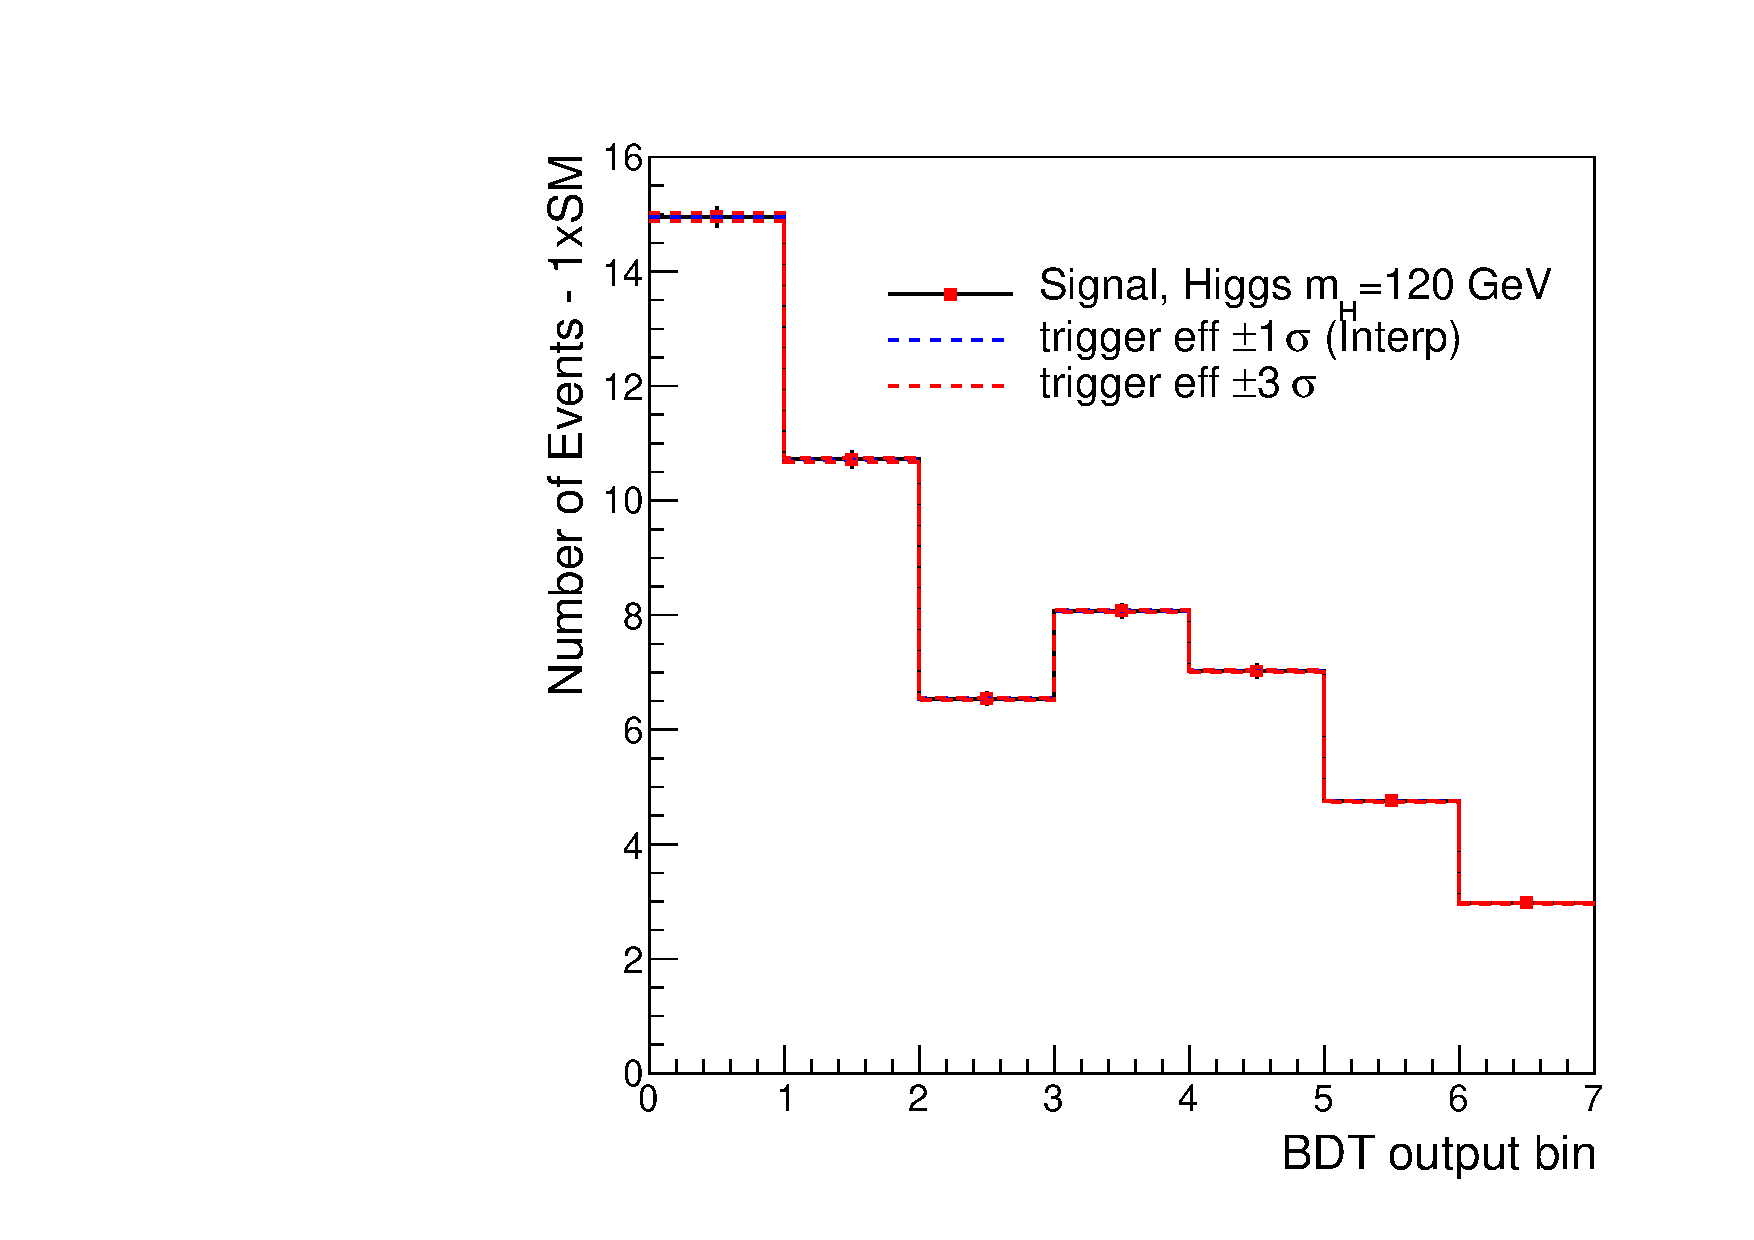
\includegraphics[width=0.45\textwidth]{hgg7TeV/sidebandMvaPlots/signalModel/systematic_interpolation_test_triggerEff}
  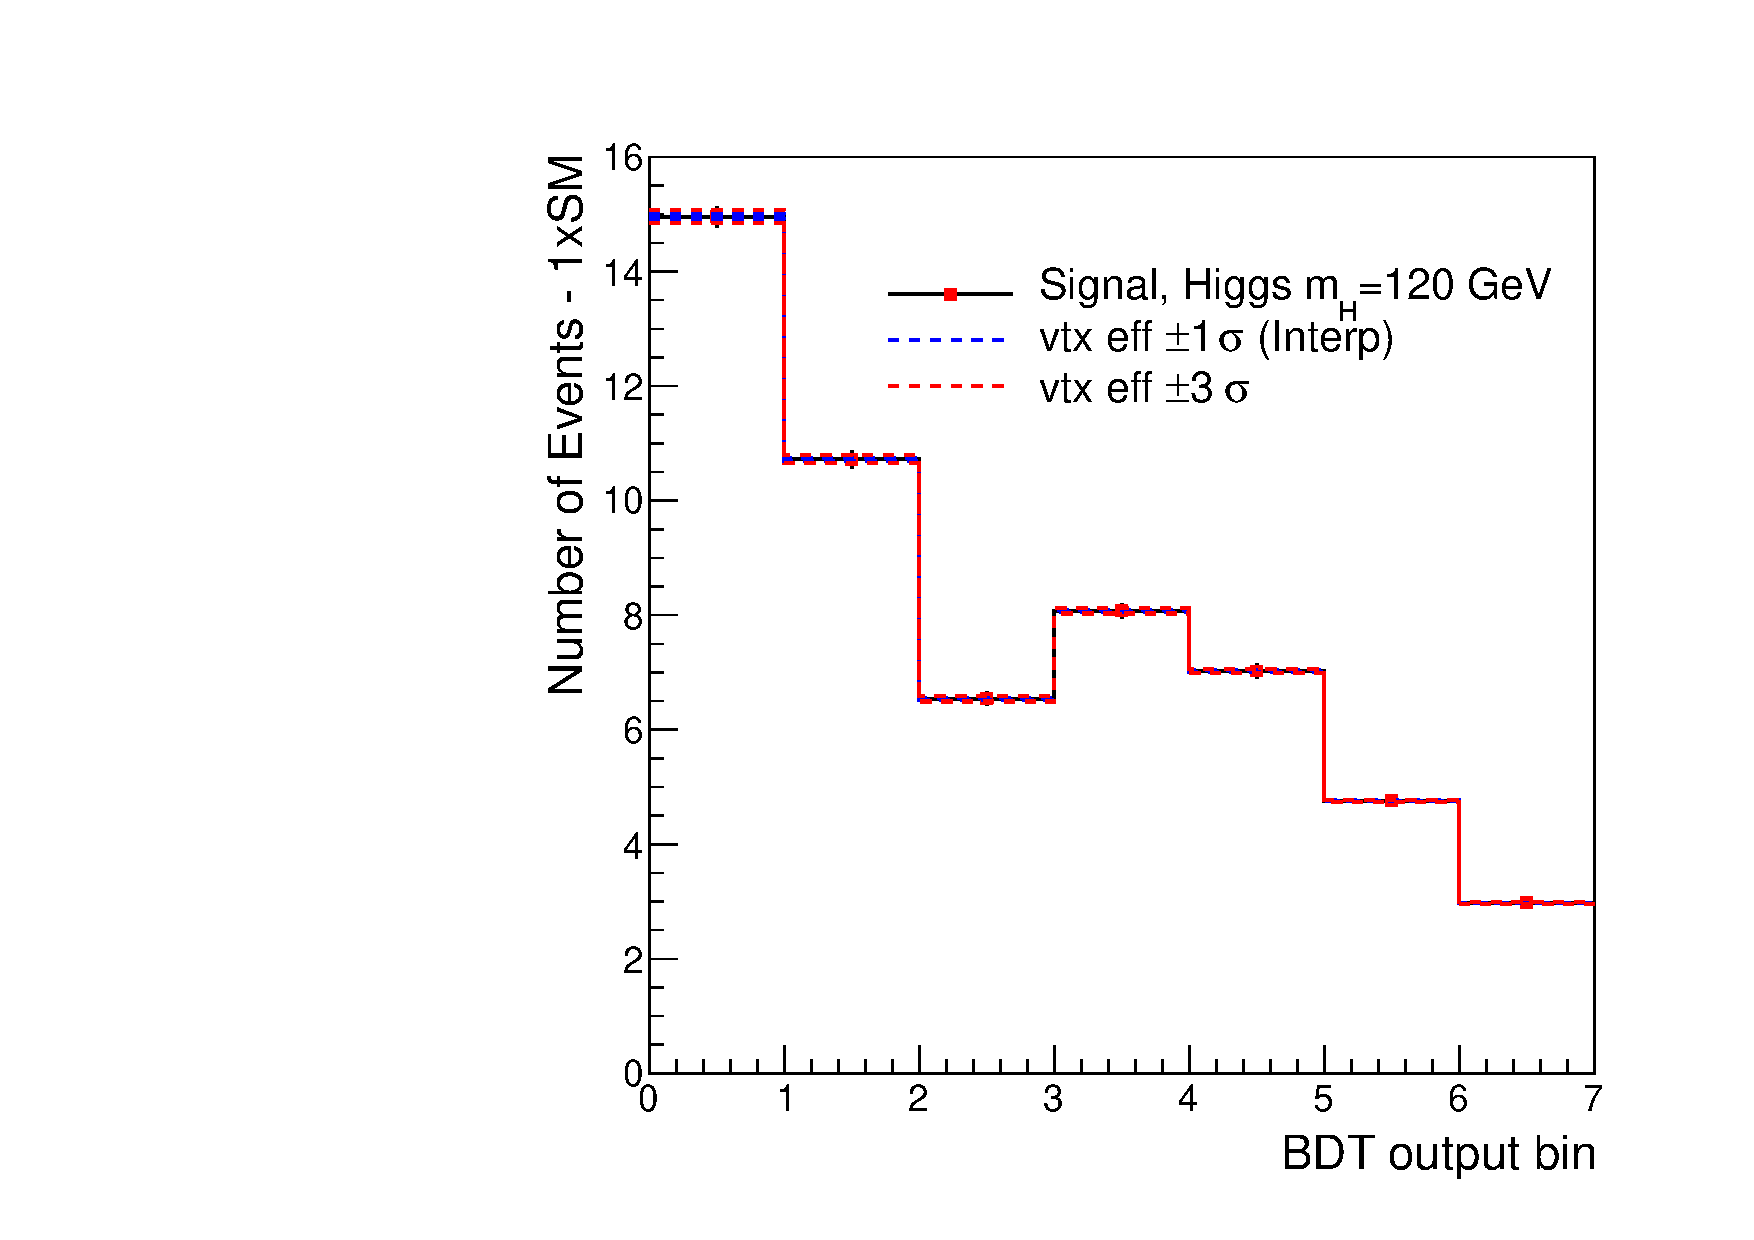
\includegraphics[width=0.45\textwidth]{hgg7TeV/sidebandMvaPlots/signalModel/systematic_interpolation_test_vtxEff}
\end{center}
\caption{Systematic uncertainties on the $ggH$ signal model. 
The effects of $\pm3\sigma$ variations 
derived in MC is shown with red dashed lines while the interpolated $\pm3\sigma$ are shown with blue.}
\label{fig:additionalsignalsys}
\end{figure}

